\hoofdstuk{Background}
\paragraaf{Lunatech Research B.V}
Lunatech provides application development services, completely based on open-source web and Java technologies and open standards. They are early adopters of new technology, and use cutting-edge frameworks and tools. To stay up-to-date, their developers have the opportunity to research, try new technologies and contribute to open-source projects. The company is dominated by software developers. Everyone (except the director) writes code, on top of which some staff have a secondary management role, and the staff who will deliver a project interact with the customer directly.

\paragraaf{Rotterdam University of Applied Sciences (Hogeschool Rotterdam)}
Rotterdam University is one of the major Universities of Applied Sciences in the Netherlands. Currently almost 30,000 students are working on their professional future at the university.
The university is divided into eleven schools, offering more than 80 graduate and undergraduate programmes in seven fields: art, technology, media and information technology, health, behaviour and society, engineering, education, and of course, business.\cite{HogeschoolRotterdam2012}

\paragraaf{Stager}
In 2011, live music venue WORM - Instituut voor Avantgardistische Recreatie hired Lunatech to build \emph{Stager}, a modern web-based resource planning and ticketing application to help manage live music events. Lunatech took the opportunity to use the relatively new Play framework to build a web application with an HTML5 and Java architecture. Stager has broad requirements ranging from high performance and security for the public ticket sales component to high usability for the internal resource planning component that will be used for hours a day by employees and being open to enhancements in the future for new customers. \cite{Lunatech2011} %todo: bron toevoegen

\subparagraaf{WORM}
WORM is een instituut voor avantgardistische recreatie te Rotterdam, bestaande uit een kunstenaarscollectief, een podium met winkel en een Parallelle Universiteit (DIY-werkplaatsen voor film, muziek en media). Geboren onder de sterren van punk, dada, fluxus, situationisme en futurisme is WORM uitgegroeid tot een eigengereide organisatie die de ‘Do-It-Yourself’ mentaliteit van hun voorouders combineert met ultra-pragmatisme, liefde voor techniek(en) en goede boekhouding. De output van WORM is film, radio, concerten, cursussen, partys, publicaties, performances, web-projecten, installaties, workshops en een opeenhoping van tactiele media en internet.WORM focust zich (blijmoedig en toch serieus) op avantgarde, middelenschaarste en opensource.\#todo: translate \cite{WORM2012} %TODO bron toevoegen

\hoofdstuk{Mobile platforms}

\paragraaf{Introduction}
% per platform: van wie is het, wat is de geschiedenis, waar wordt het gebruikt, welke achterliggende techniek drijft het?
% plaatjes homescreens of devices toevoegen, visueel maken.

The following chapter presents a concise overview of current mobile operating systems for mobile platforms, specifically smartphones and tablets.

% todo: define platform.

A smartphone can be defined as a smart phone is a next-generation, multifunctional cell phone that provides voice communication and text-messaging capabilities and facilitates data processing as well as enhanced wireless connectivity.\cite{Ni2006}

\subparagraaf{Apple iOS}
iOS is a proprietary mobile operating system, developed by Apple Inc. It was originally released in 2007 for the iPhone and iPod Touch. iOS also became the main operating system of the iPad and Apple TV.

\subparagraaf{Google Android}
Android is a opensource mobile operating system, developed by the Open Handset Alliance, led by Google and other companies.\cite{Inc.2012}

\subparagraaf{BlackBerry OS}
BlackBerry OS is a proprietary mobile operating system, developed by RIM\emph{(Research In Motion)} for its line of BlackBerry mobile devices.

\subparagraaf{Windows Phone 7}
Windows Phone 7 is a mobile operating system, developed by Microsoft as a succesor to its Windows Mobile platform.

\subparagraaf{Other platforms}
% Onder other valt Symbian. Symbian is een app platforms dus we nemen het mee:)
\subparagraaf{Java ME}
\subparagraaf{Symbian}

\paragraaf{Distribution of applications}
%todo

\paragraaf{Marketshare and trend}
% TODO: waar de stats vandaan komen,  wat ze betekenen, waarom ik ze heb gekozen, wat de alternatieven zijn((gartner 2011)
\begin{centering}
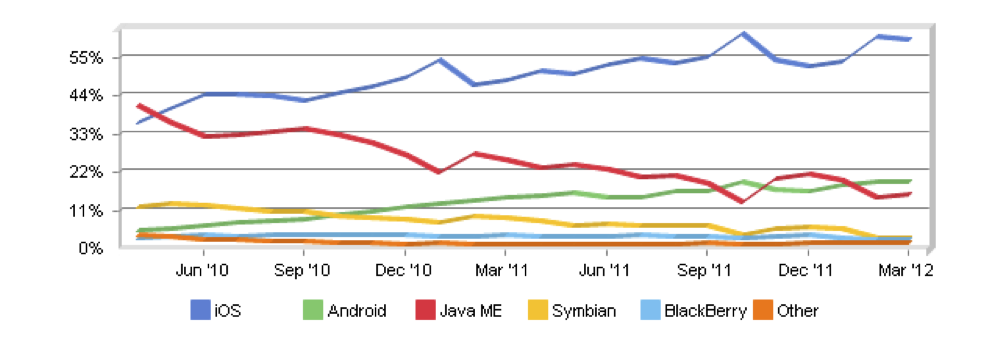
\includegraphics[scale=0.5]{images/marketsharetrendsApril10Tomay12.png}\\{World wide mobile OS Marketshare trends, April 2010 up to may 2012}\\
\end{centering}

\begin{centering}
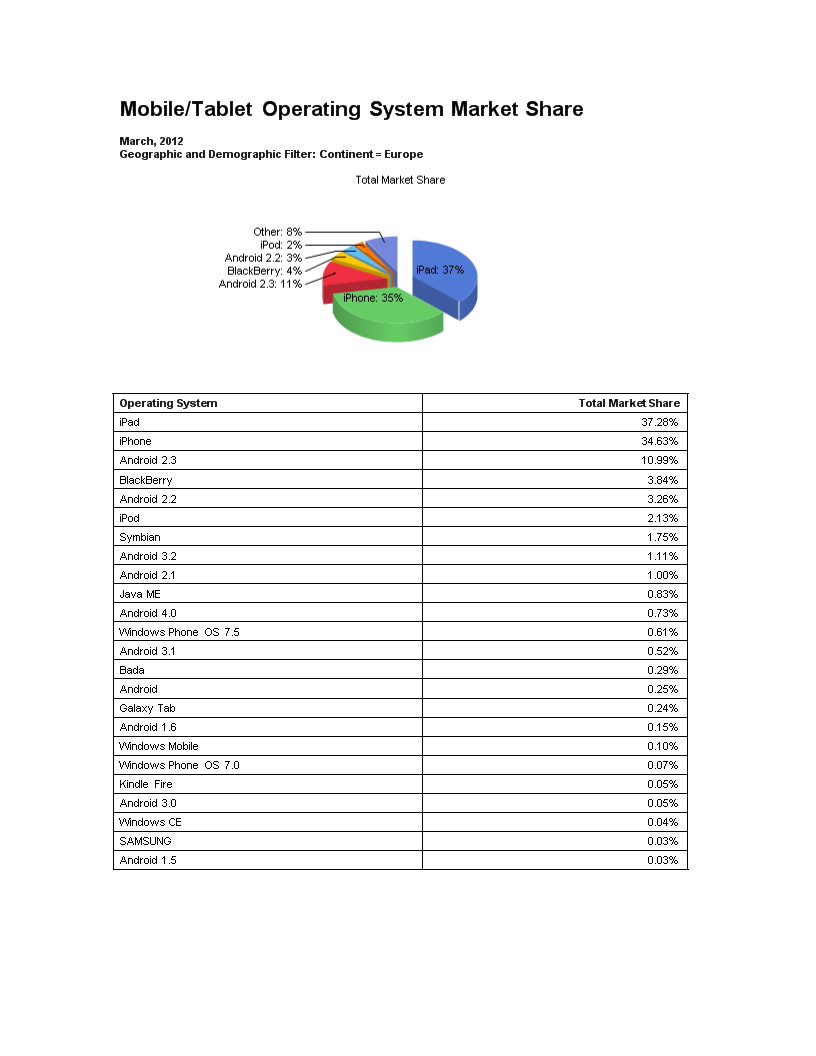
\includegraphics[scale=0.5]{images/netmarketshare_march2012.png}\\
\end{centering}

\begin{tabel}{|>\R p{\Procent{25}} | >\R p{\Procent{25}} |}{vbx}{Marketshare in the european continent as of march 2012\cite{Netmarketshare2012}}
\hline
\bf{Operating System} & \bf{Total \% Market Share}\\
\hline \hline
iOS & 74.04\\
Android & 18.36\\
BlackBerry & 3.84\\
Symbian & 1.75\\
Java ME & 0.83\\
Windows Phone & 0.68\\
Bada & 0.29\\
Windows Mobile & 0.14\\
Kindle & 0.05\\
Samsung & 0.03\\
LG & 0.01\\
ZTE & 0.00\\
Palm & 0.00\\
\hline
\end{tabel}



\hoofdstuk{Defining native}
\paragraaf{Introduction}
This chapter will define the paradigm of \emph{native look-and-feel}.

\paragraaf{Native mobile applications}
A native application is an application inherent to the platform for which it was built using techniques proprietary to the platform. For example, an iOS application is native when written in Objective-C and an Android application is written in Java.  Native applications are typically fast and can access the device's native API's.

\subparagraaf{The native look-and-feel}
When written in the native framework for a platform a mobile application receives acces to the available public libraries of the platform. These libraries include the UIKit\emph{(on iOS)} which provides the developer with a pre-fabricated set of user interface components. These can be seen as the building blocks for the graphical user interface on that platform. When used, the general style of the mobile application gains consitency to the overal user interface design of the platforms operating system. This gives an application its native look, which in turn participates to the \emph{native feel}.

%with a feeling of recognition when using the application, userinterface elements work as they expected based upon experience with using the operating system.
%todo: add some notes about the Human Interface Guidelines.

The \emph{native feel} of a mobile application can be defined as the speed in which the userinterface elements, the responsiveness of user interface elements to touch events, and smoothness of the animation in which the user interface elements are moved. A native mobile application has the advantage to hardware acceleration. This means its code has been precompiled and directly executed by the device CPU, rather than having to be interpreted by the device's browser. As a result of this the user interface elements are rendered faster and it \emph{feels} smooth.
 	

\paragraaf{Alternative mobile application types}
\subparagraaf{Web applications}
A mobile web application is an application developed with web technologies as JavaScript and HTML5 with CSS3. It is in fact nothing more than a website designed to fit on mobile devices, often they resemble the style of a native application rather than a traditional website. These applications are build with a JavaScript library to add support for scrolling and handling touch events. Touch events are handled via user interface elements provided by the library. Examples of these libraries include jQtouch, SenchaTouch.

% todo: screenshots/links neerzetten.

\subparagraaf{Hybrid applications}
A hybrid application in mobile development refers to an application which use a native shell to wrapped around web app. There are generally two forms of native shells, the first is a \emph{webview} and the second a native framework which exposes a javascript API to provide the web application access to otherwise native API's.

\subparagraaf{Webview-based hybrid applications}
A webview-based hybrid application is a webbased mobile application wrapped in a webview. A webview is a view or element which acts like a browser would, e.g. it is able to render HTML and run javascript.  It is readily available in the native libraries. The advantage of a webview-based hybrid application over an normal web application is that it can be published via the devices native application publishing platforms. e.g. a webview-based hybrid application targetted for the iPhone can be placed in the Apple appstore. 

Worklight is an example of a framework which can be used to develop webviewbased hybrid applications.

\subparagraaf{Framework hybrid applications}
A Framework based hybrid application is a webviewbased application build upon a framework which provides a Javascript API to allow the application access to otherwise native API's. The framework is written in the platforms native programming language making it possible to access the native API, such as reading contact list, composing of SMSes, full access to the location API, etc.

PhoneGap is an example of a framework which can be used to develop mixed hybrid applications.

\paragraaf{Comparison}
Web applications are quick and cheap to develop. Written entirely in HTML5, CSS and JavaScript. Executed by the mobile
browser and therefore cross - platform by default, but less powerful than native apps.
 
Hybrid Applications (Web), the app's source code consists of web code executed within a native wrapper that is provided by a framework.
 
Hybrid Applications (Mix), the developer augments the web code with a Javascript API to create unique features and
access native APIs that are not yet available via the browser, such as AR, NFC and others.
 
Native Application are platform-specific. Requires unique expertise and knowledge. Pricey and time consuming to develop but
 delivers the highest user experience of all approaches.

\begin{centering}
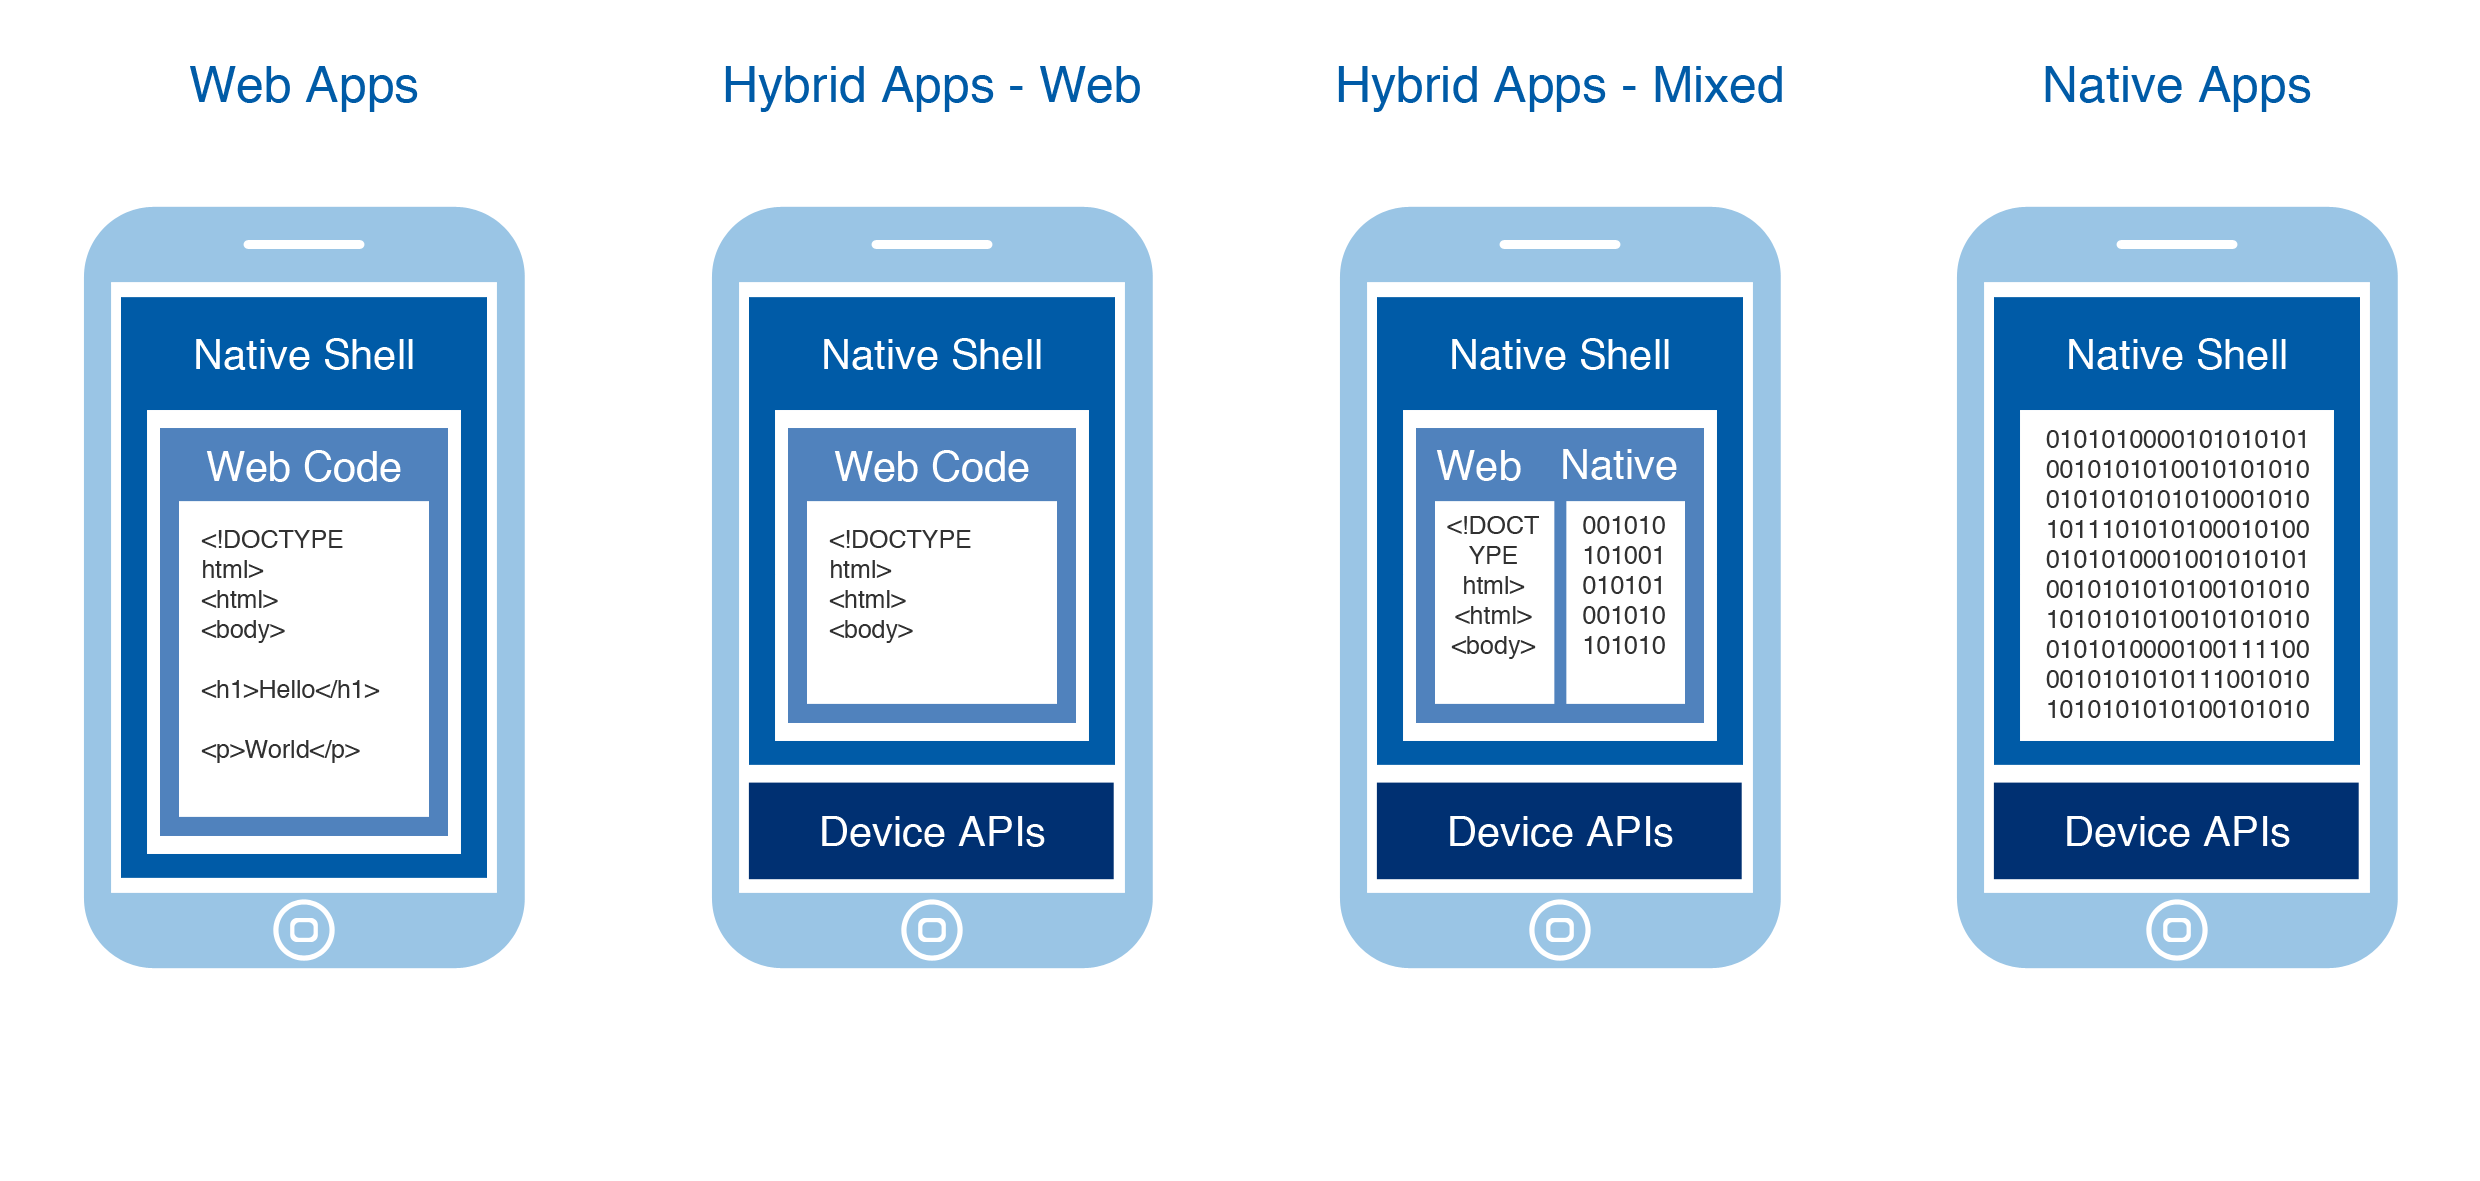
\includegraphics[scale=0.5]{images/apptypesdefined.png}\\{Different types of mobile applications\cite{IBM-Worklight2012}}\\
\end{centering}

\hoofdstuk{Exsisting solutions to Cross-platform Mobile Application Development}
\paragraaf{Introduction}
In todays industry there exist several cross-platform mobile application development framework which offer a solution to cross-platform problem. All of these framework provide a custom solution for crossing the bridge between platforms. In order determine which one should be adopted by Lunatech for mobile development the following criteria have been determined for comparisson:

\begin{enumerate}
\item \emph{Platform support}\\
Which platforms and their versions are supported by the framework.
\item \emph{Native UI support}\\
Whether or not native user interface elements are supported for each supported platform.
\item \emph{Programming language}\\
Which programming language is used to develop using the framework.
\item \emph{IDE} (Intergrated Development Environment)\\
Which IDE can be used to develop using with the framework.
\item \emph{License type}\\
Which license types are available.
\item \emph{Application type}\\
Which type of mobile application is produced using this framework.
\end{enumerate}

The cross-platform criterium is based on Lunatechs requirement to build mobile applications for the operating systems have at least a 10 percent marketshare in the European continent. Second  comes the support for native user interface elements. Together these criteria form the essence of the main research question: "\emph{How to develop a cross-platform mobile application while retaining the native look-and-feel?}"
The remaining criteria are of secondary importance, they will provide more detailed means to compare the frameworks which offer native user interface support.

The following solutions have been choosen for review: \emph{Titanium, Rhodes, Worklight and MoSync}. These are derived from the list Existing solutions\footnote{see attachment: \emph{Existing solutions}} %todo!


\paragraaf{Appcelerator Titanium}
Appceleator Titanium is an commericially supported opensource platform for developing cross-platform mobile applications. It was introduced by Appcelerator Inc in December 2008. Built upon the Eclipse IDE Titanium offers a Javascript API to native proxy classes which allow the developer to generate truely native cross-platform mobile applications. 
%todo uitleggen proxy classes.

\subparagraaf{Platform support and native capability}
As of may 2012 Titanium supports iOS and Android. Next to building a native application for these platforms Titanium offers the option to generate a web application. 
Support for Research in Motion (BlackBerry) is in active (however closed from public) development. May first 2012 Appcelerator announced that it is extending its core value of cross-platform native application development beyond iOS and Android, on to RIM's BlackBerry devices.\cite{Asher2012}

\subparagraaf{Techniques and tools}
TitaniumStudio is an Eclipse based IDE with integration the propriatory mobile SDKs and simulators. For iOS this means Titanium requires Xcode with the iOS SDK to be installed, for Android the Android SDK and the Android AVD\footnote{AVD: Android Virtual Device (device simulator)} are required.

Titanium application are primarily written in JavaScript but be augmented with HTML \& CSS. 

Prior to compiling an application Titanium loads the JavaScript files into a single JavaScript Evaluator. 

\subparagraaf{Application type}
Applications built with Titanium can be devided into two types.

\begin{itemize}
	\item
	Framework hybrid applications
	\item
	Native applications
\end{itemize}

\subparagraaf{Philosophy}
The goal of Titanium is to provide a high level, cross-platform JavaScript runtime and API for mobile development.\cite{Whinnery2012}

\paragraaf{Rhodes}
Rhodes is an open source Ruby-based framework to build native applications for all major smartphone operating systems (iPhone, Android, RIM, Windows Mobile and Windows Phone 7). These are true native device applications (not mobile web applications) which work with synchronized local data and take advantage of device capabilities such as GPS, PIM contacts and calendar and the camera. %todo: herfomuleren

\subparagraaf{Platform support and native capability}
iOS, Android, BlackBerry, Symbian, Windows Mobile
\subparagraaf{Techniques and tools}
Eclipse based studio, Ruby \& HTML
\subparagraaf{Application type}


\paragraaf{Worklight}
Worklight Studio is an eclipse based IDE for the cross-platform development of mobile applications. Worklight Studio was introduced in 200x by Worklight Inc. In early 2012 Worklight Inc. became an IBM company. Worklight Studio offers mobile development trough the use of webtechnologies such as HTML5, and Javascript.

\subparagraaf{Platform support and native capability}
iOS, Android, BlackBerry, Windows Mobile	
\subparagraaf{Techniques and tools}
Eclipse plugin, HTML5, CSS, Javascript
\subparagraaf{Application type}
Hybrid web

\paragraaf{MoSync}
The MoSync mobile SDK offers cross-platform development trough the use of webtechnologie or C/C++.
\subparagraaf{Platform support and native capability}
\subparagraaf{Techniques and tools}
\subparagraaf{Application type}

\paragraaf{PhoneGap}
\paragraaf{Sencha Touch}
\paragraaf{jQTouch}

\paragraaf{Comparisson}



\hoofdstuk{Developing cross-platform native applications with Titanium}
\paragraaf{Inner workings}
basically, at runtime, your application consists of three major components – your JavaScript source code (inlined into a Java or Objective-C file and compiled as an encoded string), the platform-specific implementation of the Titanium API in the native programming language, and a JavaScript interpreter that will be used to evaluate your code at runtime (V8 (default) or Rhino for Android, or JavaScriptCore for iOS). Except in the browser, of course, where the built-in JavaScript engine will be used.When your application is launched, a JavaScript execution environment is created in native code, and your application source code is evaluated. Injected into the JavaScript runtime environment of your application is what we call “proxy” objects – basically, a JavaScript object which has a paired object in native code. Colloquially we will often refer to “JavaScript land” and “native land” in a Titanium application, as they are kind of parallel universes to one another. The proxy object exists both in JavaScript land and native land, and serves as the “bridge” between the two.
In your JavaScript code, when you call a function on the global Titanium or Ti object, such as var b = Ti.UI.createButton({title:'Poke Me'});, that will invoke a native method that will create a native UI object, and create a “proxy” object (b) which exposes properties and methods on the underlying native UI object to JavaScript.
UI components (view proxies) can be arranged hierarchically to create complex user interfaces. Proxy objects which represent an interface to non-visual APIs (like filesystem I/O or database access) execute in native code, and synchronously (or asynchronously for APIs like network access) return a result to JavaScript. \cite{Whinnery2012}

\hoofdstuk{Case study}
\paragraaf{Stager app}
\paragraaf{Stager application requirements}
\subparagraaf{Events}
\subparagraaf{Notifications}
\subparagraaf{Tickets}
\subparagraaf{i18n}
\subparagraaf{Mobile payment}
\paragraaf{Used techniques and methodologies}
\subparagraaf{Javascript}
\subparagraaf{CommonJS}
\subparagraaf{JSON}
\subparagraaf{Playframework}
\subparagraaf{Java}


%\paragraaf{Titanium modules}
%\paragraaf{Stager service modules}









